% Halo correlation multipoles of the 512^3 production boxes with the gravitational-redshift shift.
% Figures and table: make_ximult_box_figures.py; data: data/box512_L200_L500_L1000/L<L>_out100_ximult.npz.

\paragraph{Measurement.} \fp{scripts/post-process/halo_xi_multipoles.py} (pipeline stage \texttt{ximult}) on the
three matched-seed $512^3$ boxes of Section~\ref{sec:boxsize} at $z = 0$ (output 100): host halos in the mass bins of
the stacked profiles ($M_{\rm vir}$), pair counts in $(s, \mu)$ with Corrfunc \texttt{DDsmu} from the
\texttt{adematti/Corrfunc} fork (branch \texttt{desi}: signed $\mu$, so the odd multipoles survive), analytic random
pairs of the periodic box, $s = 0$--$100$\,\Mpch{} in 2\,\Mpch{} bins, 200 $\mu$ bins, multipoles $\ell = 0\ldots4$.
Each halo is moved along the line of sight by $v_{\rm los}/(aH)$ (\emph{rsd}), by $v_g/(aH)$ with $v_g = -\phi/c$
and $\phi = \phi_{r_s}$ (mean particle potential within $r_s$, from \texttt{.vpot}; $\phi_{0.5R_{\rm vir}}$ where
undefined) (\emph{grav}), or by both. The plane-parallel line of sight is $x$, $y$ and $z$ in turn; the pair counts
are averaged over the three, and each line of sight is also stored on its own. The potential effect is the difference
of two spaces with the same halos, $\xi_\ell^{\rm grav}-\xi_\ell^{\rm real}$ and $\xi_\ell^{\rm rsd+grav}-\xi_\ell^{\rm
rsd}$, with its own (paired) jackknife error over $3^3$ sub-cubes of the A halos, for the mean and for each line of
sight. Convention: $\mathbf s = \mathbf x_B - \mathbf x_A$, $\mu = s_{\rm los}/s$; a B population moved by $+\delta$
gives $\xi_1 = -\delta\, d\xi_0/ds$. Halos in deeper potentials have larger $v_g$, so with B the heavier bin the
gravitational dipole is positive where $\xi_0$ falls with $s$. Cost: 18--33\,s and 0.3--0.5\,GB per box on 32 cores
(jobs 2538076--78, 16 Nov 2026). Halos without a potential (2070, 3817, 5625 in L200, L500, L1000) are left out of
every space.

\paragraph{Mean shift estimate.} If the gravitational redshift only moved each population as a whole, by
$\delta = \langle v_g\rangle/(aH)$, the dipole would be $-(\delta_B-\delta_A)\, d\xi_0^{\rm real}/ds$ (dotted
curves). The mean $v_g$ per bin is 2.0--3.2, 3.7--4.0, 7.6--8.2 and 16.2--16.9\,km\,s$^{-1}$ (bins 0--3; the
lowest bin differs in L1000 because it is incomplete there), so $\delta_B - \delta_A$ is 0.04--0.13\,\Mpch{} for the
cross pairs (Table~\ref{tab:ximult512}).

\begin{figure}[H]
\centering
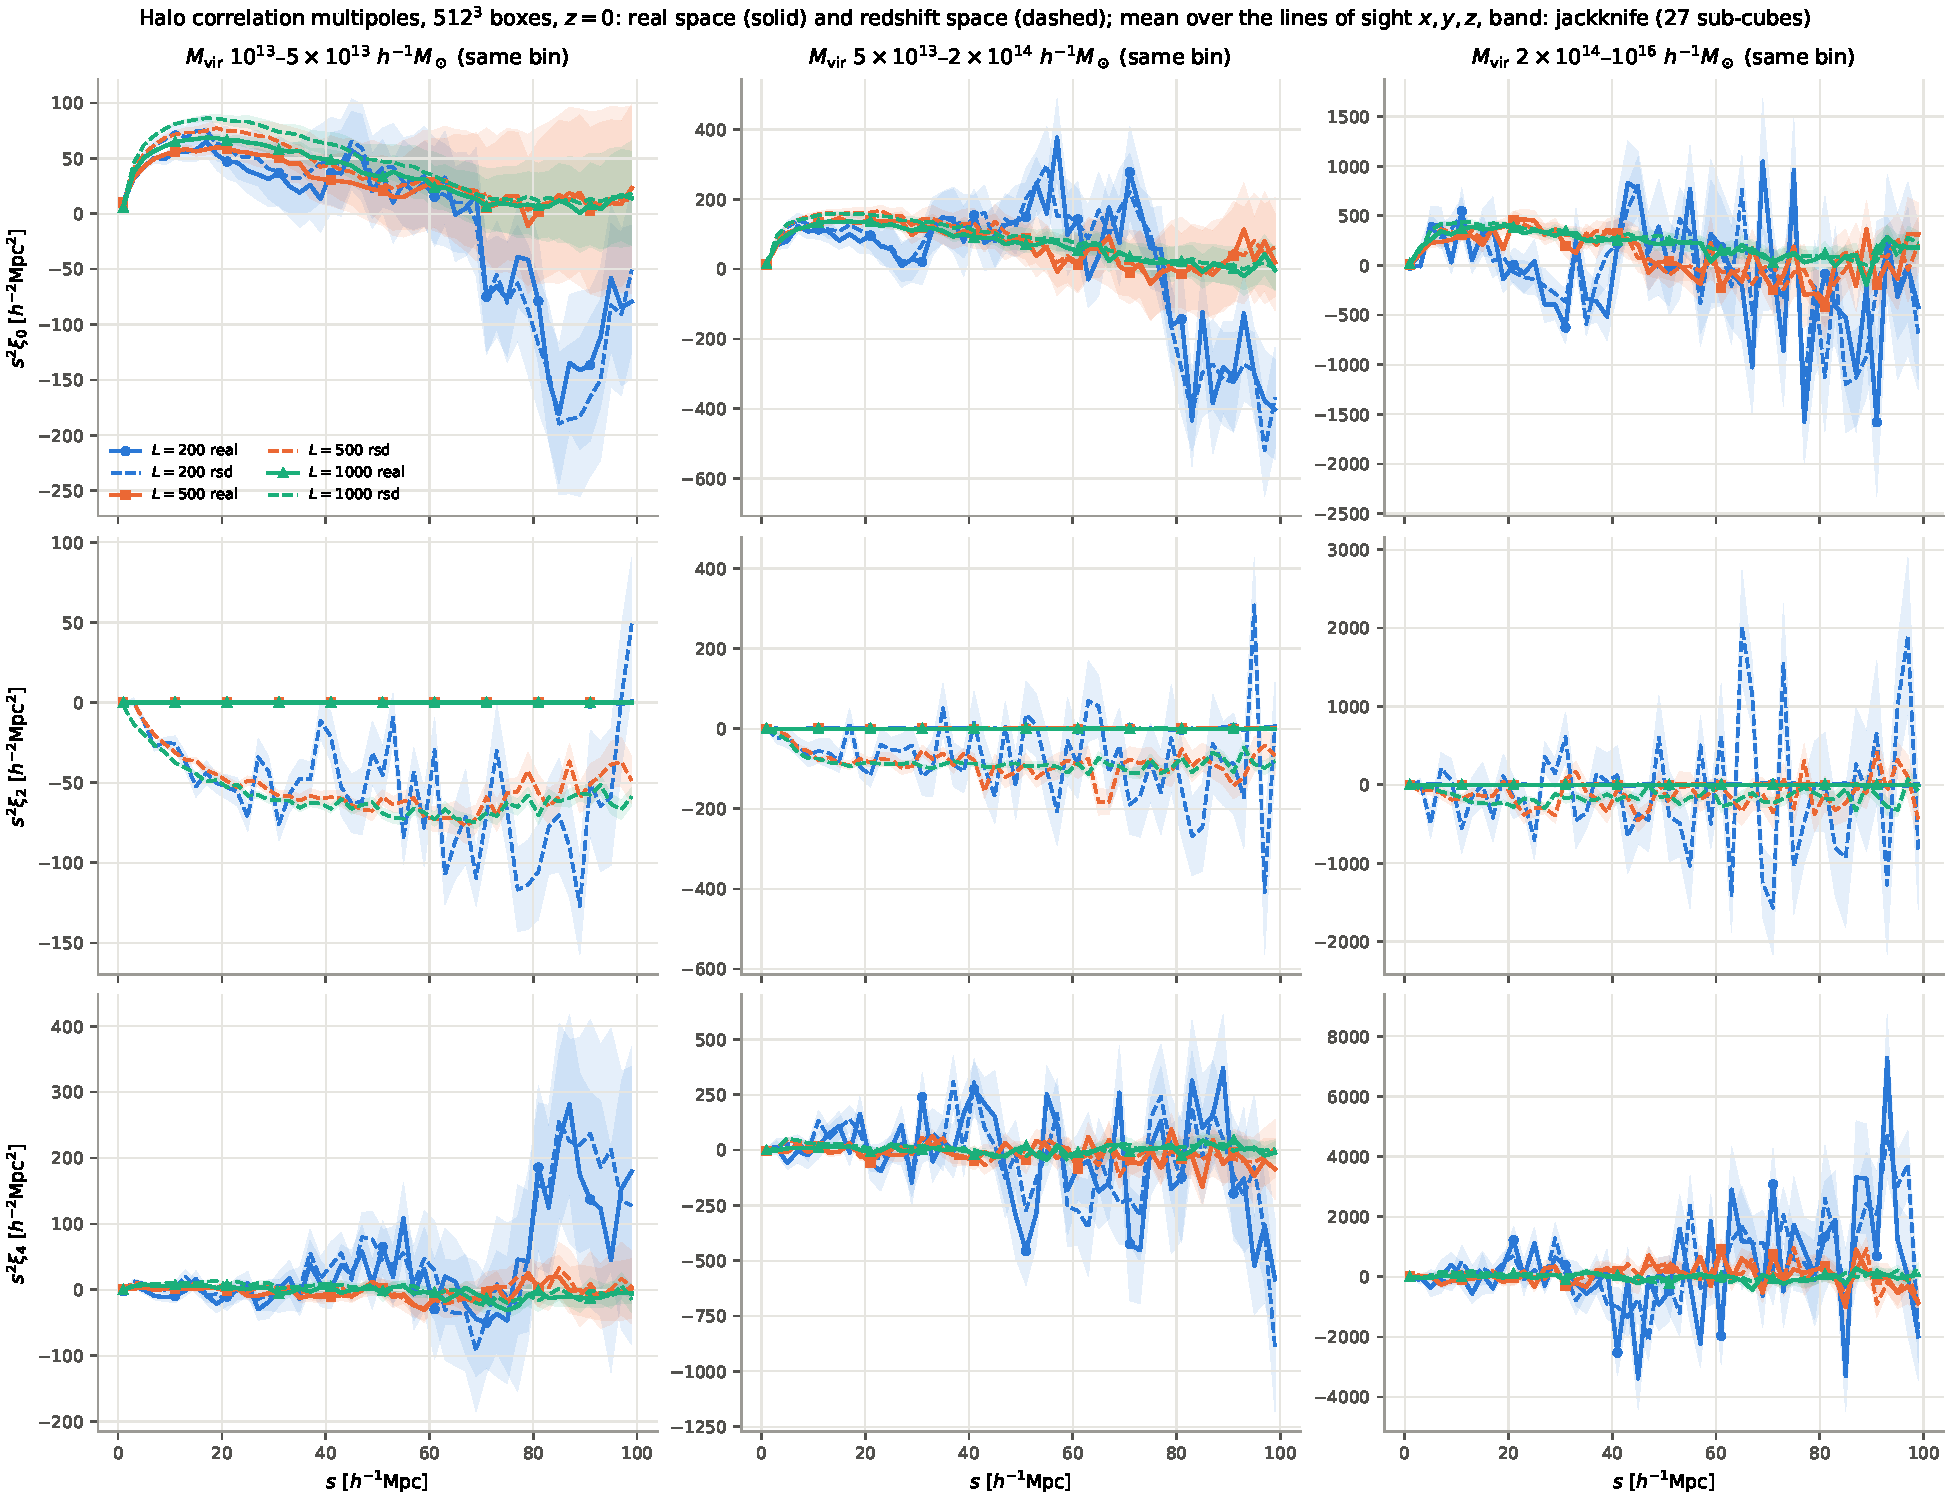
\includegraphics[width=\textwidth]{figs/ximult512_even.pdf}
\caption{Even multipoles $s^2\xi_0$, $s^2\xi_2$, $s^2\xi_4$ of same-bin halo pairs in real space (solid) and redshift
space (dashed), mean over the lines of sight $x$, $y$, $z$, with jackknife bands, in the three boxes.}
\label{fig:ximult512_even}
\end{figure}

\begin{figure}[H]
\centering
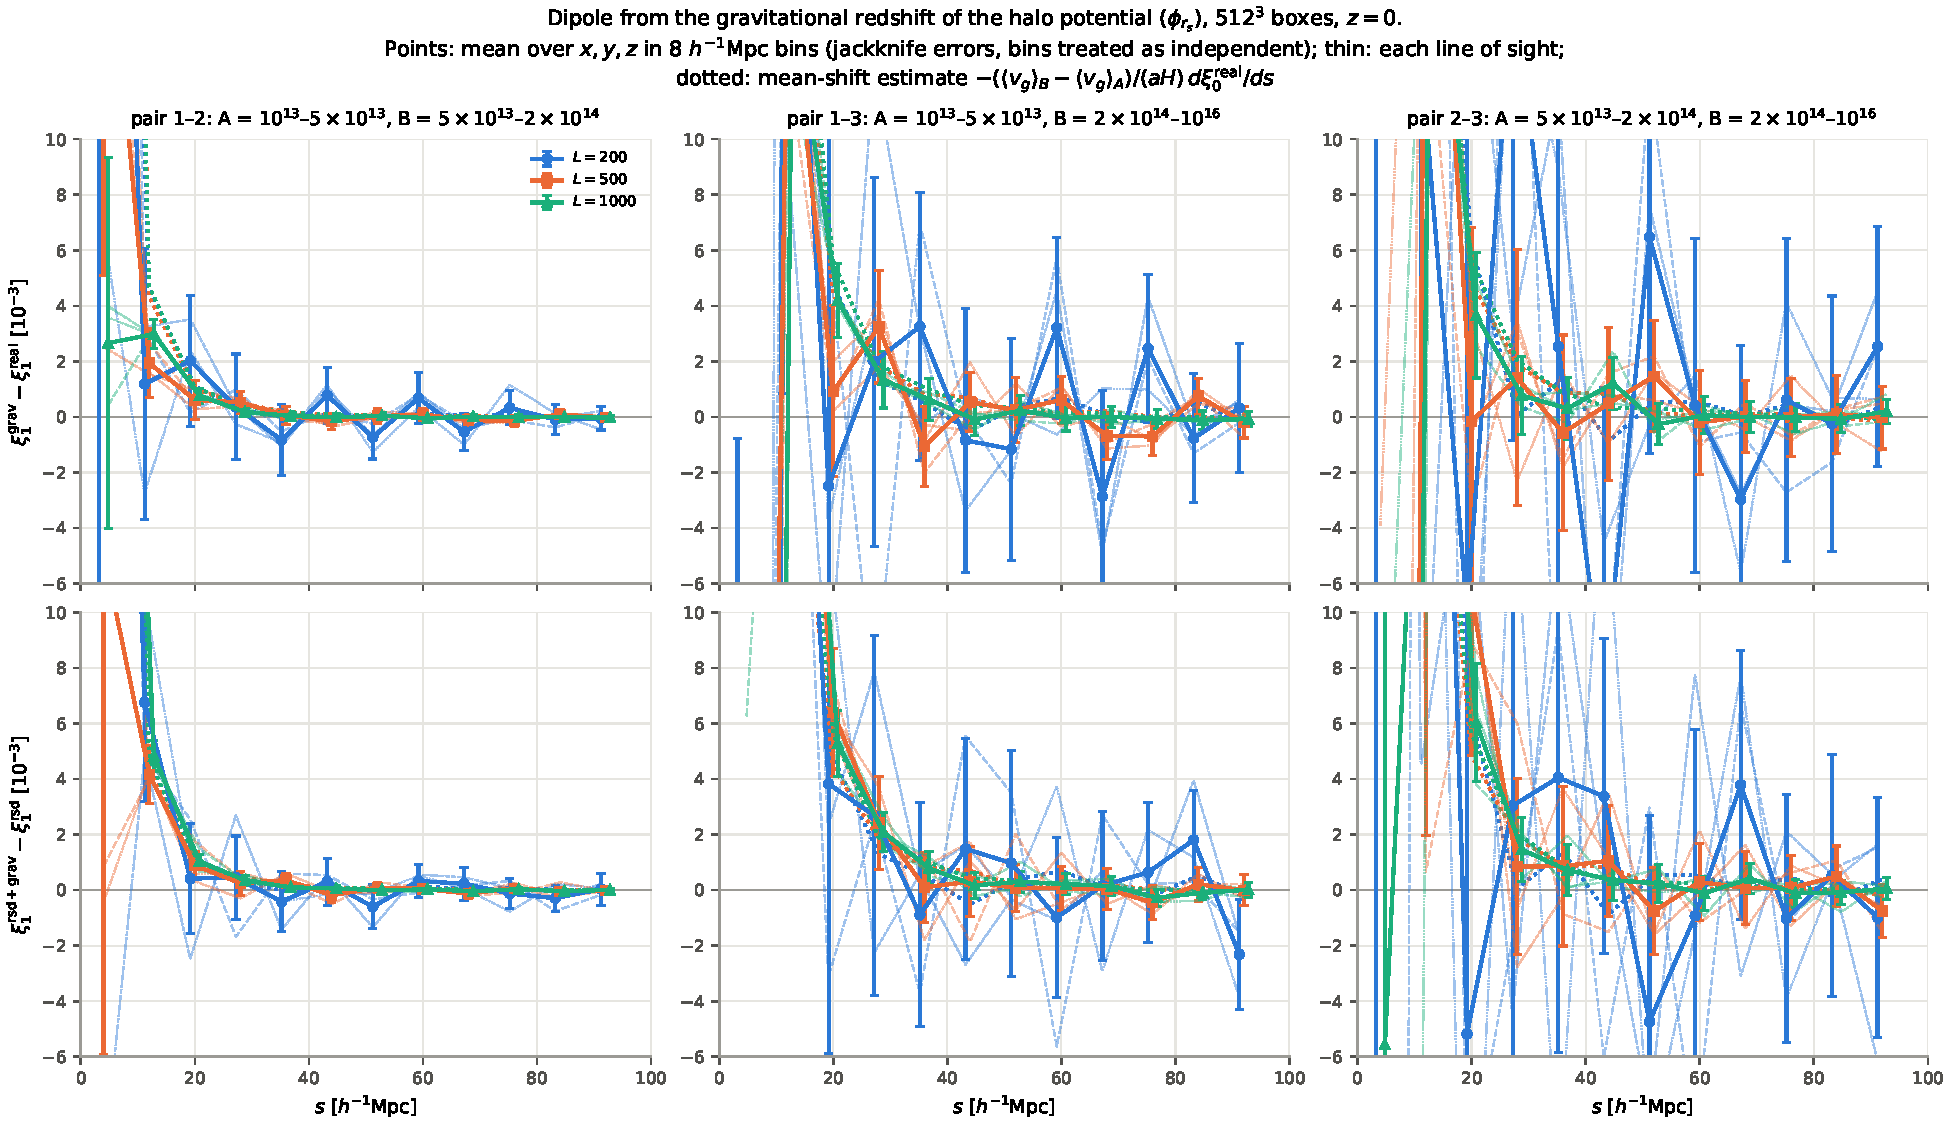
\includegraphics[width=\textwidth]{figs/ximult512_dipole.pdf}
\caption{Dipole from the gravitational redshift, $\xi_1^{\rm grav}-\xi_1^{\rm real}$ (top) and
$\xi_1^{\rm rsd+grav}-\xi_1^{\rm rsd}$ (bottom), for the three cross pairs of the upper mass bins. Points: mean over
the lines of sight averaged in 8\,\Mpch{} bins (four 2\,\Mpch{} bins; errors combined as if the bins were
independent, which underestimates them somewhat). Thin lines: each line of sight. Dotted: mean-shift estimate.}
\label{fig:ximult512_dipole}
\end{figure}

\begin{table}[H]
\centering\footnotesize
% written by make_ximult_box_figures.py
\begin{tabular}{ccccccc}
\toprule
pair & $L$ & $N_A$, $N_B$ & $\Delta\delta$ [$10^{-3}\,h^{-1}$Mpc] & $\xi_1^{\rm grav}-\xi_1^{\rm real}$ & $x$, $y$, $z$ & mean-shift est. \\
\midrule
1–2 & 200 & 3151, 526 & 39.38 & $-0.25 \pm 0.89$ & +0.21, -0.97, -0.01 & $+0.33$ \\
1–2 & 500 & 47725, 8168 & 42.21 & $+0.20 \pm 0.22$ & +0.21, +0.23, +0.04 & $+0.44$ \\
1–2 & 1000 & 220664, 62349 & 39.48 & $+0.25 \pm 0.11$ & +0.33, +0.20, +0.20 & $+0.57$ \\
\midrule
1–3 & 200 & 3151, 76 & 124.67 & $+0.55 \pm 3.51$ & +2.42, +0.94, -0.14 & $+1.32$ \\
1–3 & 500 & 47725, 1146 & 128.72 & $+0.55 \pm 1.04$ & +0.50, +0.98, +0.89 & $+1.81$ \\
1–3 & 1000 & 220664, 9175 & 130.36 & $+1.78 \pm 0.52$ & +1.91, +1.46, +1.95 & $+2.50$ \\
\midrule
2–3 & 200 & 526, 76 & 85.29 & $-1.73 \pm 8.07$ & +5.75, +8.20, +5.93 & $+0.59$ \\
2–3 & 500 & 8168, 1146 & 86.51 & $+0.70 \pm 2.47$ & +1.03, +0.99, +0.72 & $+2.00$ \\
2–3 & 1000 & 62349, 9175 & 90.87 & $+1.75 \pm 0.77$ & +2.08, +1.85, +1.00 & $+2.36$ \\
\bottomrule
\end{tabular}

\caption{Gravitational dipole $\xi_1^{\rm grav}-\xi_1^{\rm real}$ in units of $10^{-3}$, inverse-variance weighted
mean over $s = 10$--$40$\,\Mpch{} (jackknife errors of the 2\,\Mpch{} bins, treated as independent): mean over the
lines of sight with error, each line of sight, and the mean-shift estimate averaged with the same weights.
$\Delta\delta = (\langle v_g\rangle_B-\langle v_g\rangle_A)/(aH)$.}
\label{tab:ximult512}
\end{table}

\paragraph{Results.} \emph{Even multipoles} (Fig.~\ref{fig:ximult512_even}): the three boxes agree in real and
redshift space within the errors up to $\sim$40\,\Mpch; the redshift-space monopole is enhanced and the quadrupole
negative (Kaiser squashing), and $\xi_4$ is consistent with zero for these bins. Beyond $\sim$50\,\Mpch{} the L200
monopole drops below the larger boxes, the finite-box deficit of Section~\ref{sec:boxsize}; its top bin (76 halos) is
noise. \emph{Dipole} (Fig.~\ref{fig:ximult512_dipole}, Table~\ref{tab:ximult512}): only L1000 has the volume to
detect it, $(1.78\pm0.52)\times10^{-3}$ for pair 1--3 and $(1.75\pm0.77)\times10^{-3}$ for 2--3 between 10 and
40\,\Mpch{} (3.4 and 2.3$\sigma$, errors from bins treated as independent), $(0.25\pm0.11)\times10^{-3}$ for 1--2.
The three lines of sight agree with each other within their errors. The signal is 50--75\% of the mean-shift estimate
in L1000 (1.78 against 2.50, 1.75 against 2.36, 0.25 against 0.57); at $256^3$ a potential shift scaled by 50 also
gave 0.5--1.2 times the mean-shift prediction (guide \fp{docs/pkdgrav3_pipeline_pawna.md}, section 14). In L200 and L500 the dipole is consistent both with zero and with the
estimate. With redshift-space distortions included (bottom row) the potential effect on the dipole is similar. It grows
toward small $s$, where $\xi_0$ is steep; below $\sim$8\,\Mpch{} halo exclusion dominates.

\subsection{Dependence on the halo potential used}
\label{sec:ximult512phi}
% Figures and table: make_ximult_phi_figures.py; data: data/box512_L200_L500_L1000/L<L>_out100_ximult_phiall.npz.

\paragraph{Measurement.} The same measurement (same halos, mass bins, lines of sight, $s$ and $\mu$ bins, jackknife)
repeated with the shift $v_g = -\phi/c$ taken from each of the twelve potential columns of the \texttt{.vpot}
catalogue in turn (\fp{halo_xi_multipoles.py --phi <12 columns> --los x,y,z}; pawna job 2539117, 24 Nov 2026, 32
cores, 3.5\,min and 2.6\,GB per box, 26 spaces: real, rsd, and grav and rsd+grav for each column). Five columns are
the mean particle potential within a sphere of radius $r_s$, $0.5R_{\rm vir}$, $R_{\rm vir}$, $1.5R_{\rm vir}$ and
$R_{200b}$; seven are the Gaussian-smoothed potential grid of the VAHC scales at the halo, $2$, $4$, $6$, $8\,R_{200b}$
and 2, 3, 5\,\Mpch{} (\fp{vahc_fast.py}). Where a column is undefined the halo takes $\phi_{0.5R_{\rm vir}}$, as
before: for $\phi_{r_s}$ 23\% of the halos above $2\times10^{12}$\,\Msunh{} in L500 and 29\% in L1000 (empty $r_s$
sphere; none in L200), for the grid columns at most 0.25\% (L1000, $2R_{200b}$). The real- and redshift-space
multipoles and the $\phi_{r_s}$ spaces reproduce the run above exactly (largest difference 0), so every column is
measured on the same halos. The outputs are archived with the runs
(\fp{/storage/shadab/sahyadri_sims/halos/Sahyadri_L<L>N512/default512/r1/xcorr/out_100_ximult_phiall.npz}, listed in
the run's \fp{MANIFEST.json} and \fp{SHA256SUMS}, read-only).

\begin{figure}[H]
\centering
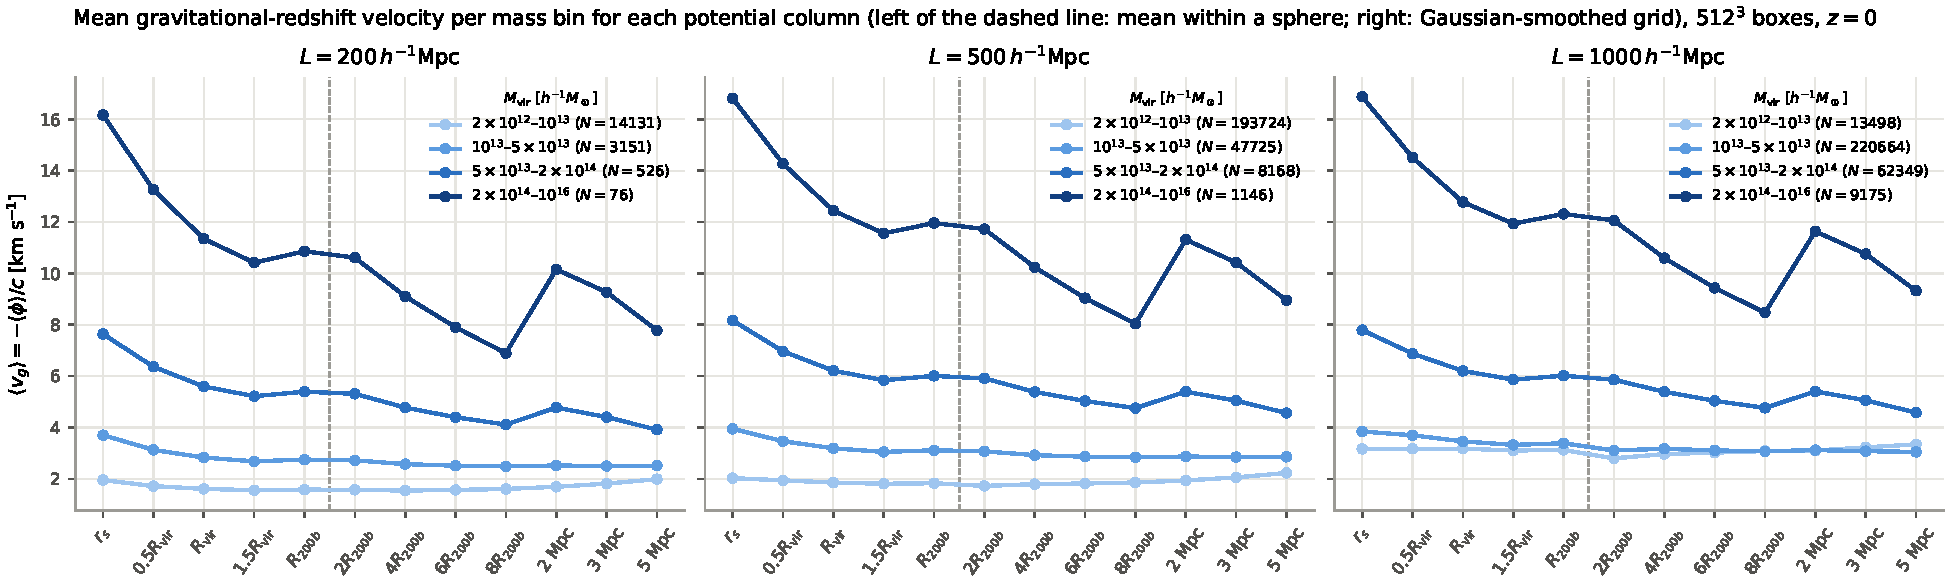
\includegraphics[width=\textwidth]{figs/ximult512_phi_vg.pdf}
\caption{Mean $v_g = -\phi/c$ of each mass bin for the twelve potential columns. Left of the dashed line: mean within
a sphere; right: Gaussian-smoothed grid. The lowest bin of L1000 (13\,498 halos against 220\,664 in the next) is
incomplete there: its halos have 3--15 particles.}
\label{fig:ximult512_phi_vg}
\end{figure}

\begin{figure}[H]
\centering
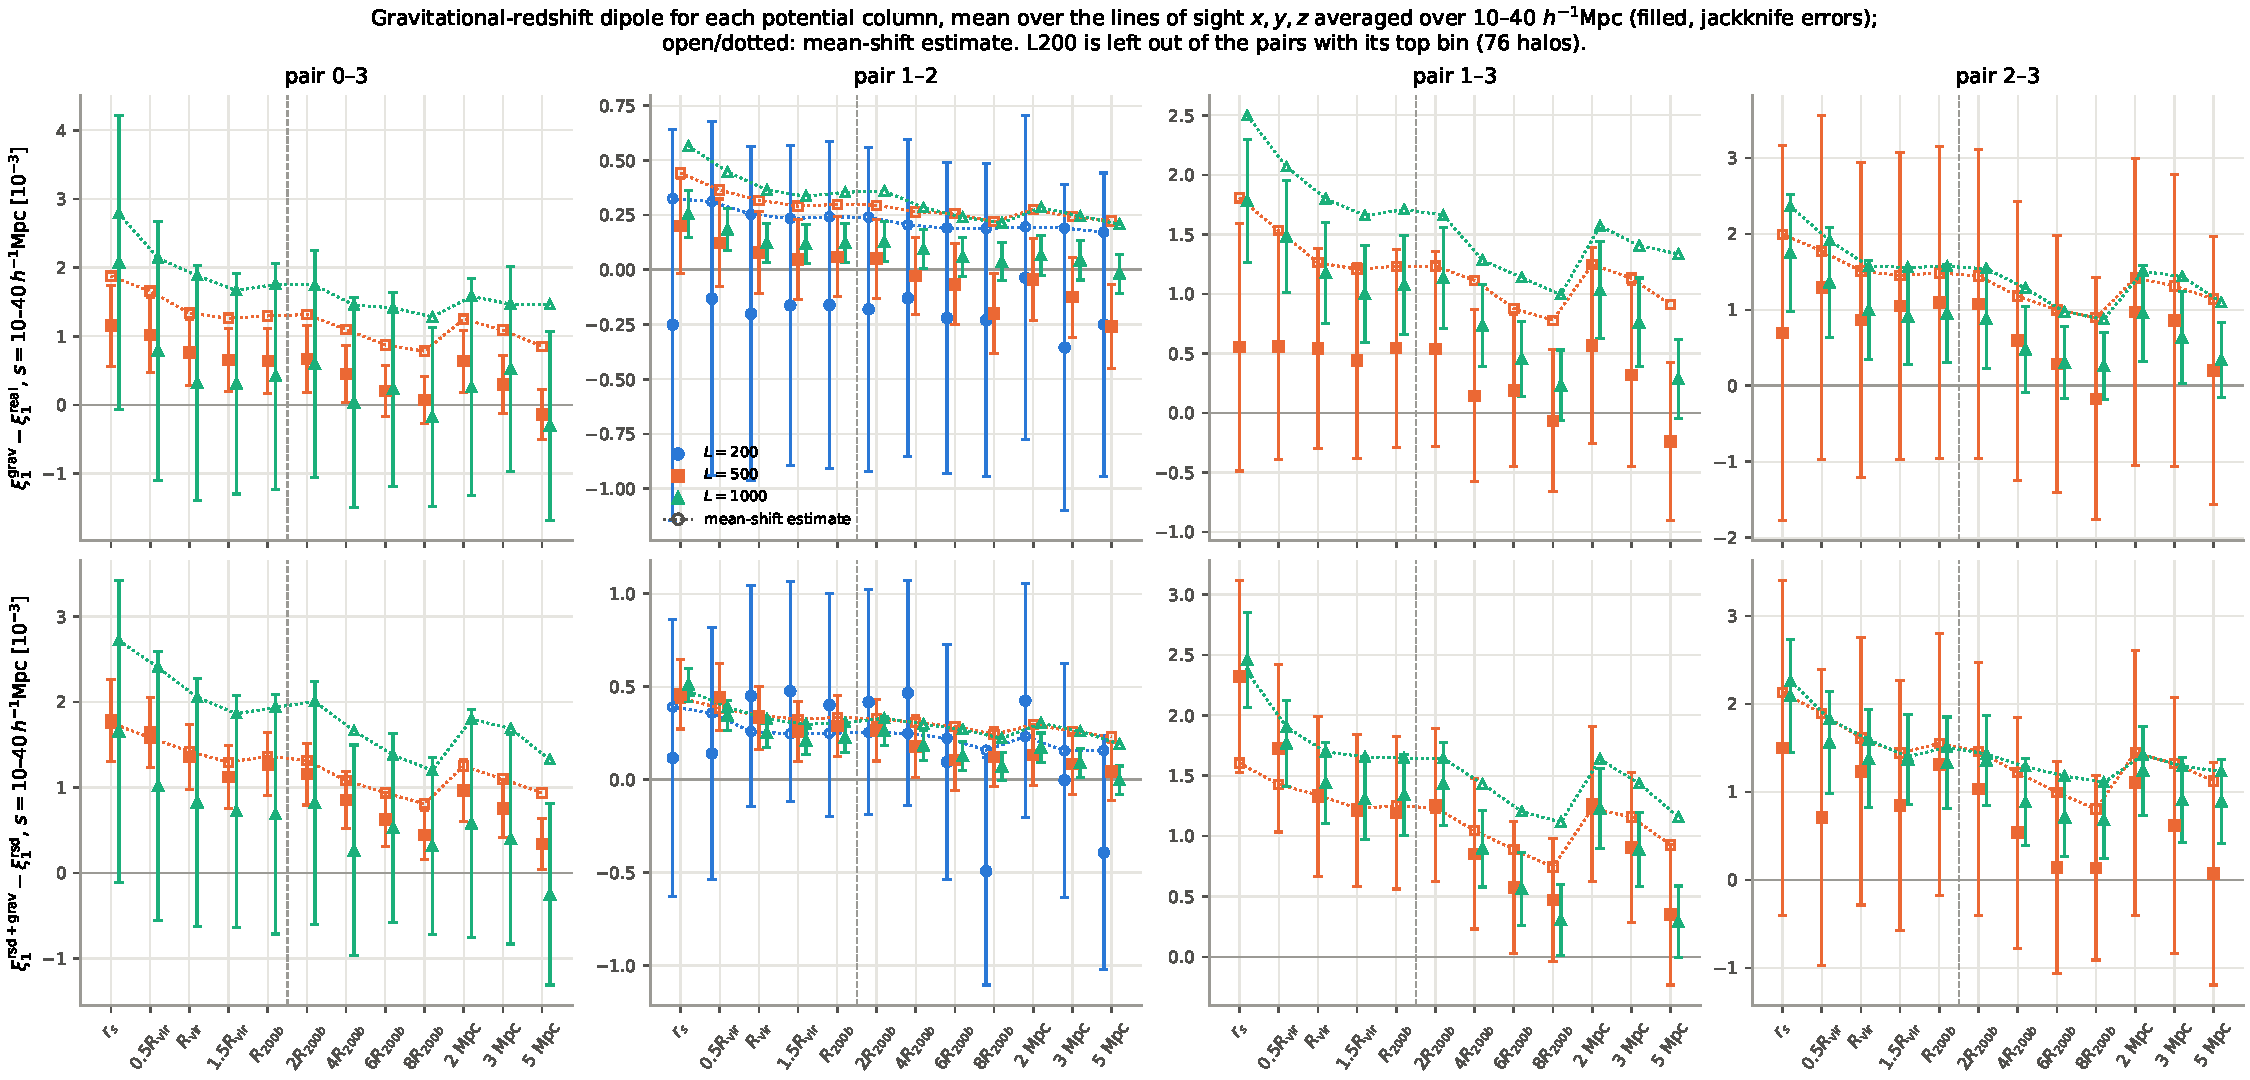
\includegraphics[width=\textwidth]{figs/ximult512_phi_dipole.pdf}
\caption{Gravitational dipole averaged over $s = 10$--$40$\,\Mpch{} (as Table~\ref{tab:ximult512}) for each potential
column: $\xi_1^{\rm grav}-\xi_1^{\rm real}$ (top), $\xi_1^{\rm rsd+grav}-\xi_1^{\rm rsd}$ (bottom), four cross pairs.
Filled: measured, mean over the lines of sight, jackknife errors of the 2\,\Mpch{} bins treated as independent; open,
dotted: mean-shift estimate with the same weights. L200 is left out of the pairs with its top bin (76 halos, jackknife
errors not reliable).}
\label{fig:ximult512_phi_dipole}
\end{figure}

\begin{figure}[H]
\centering
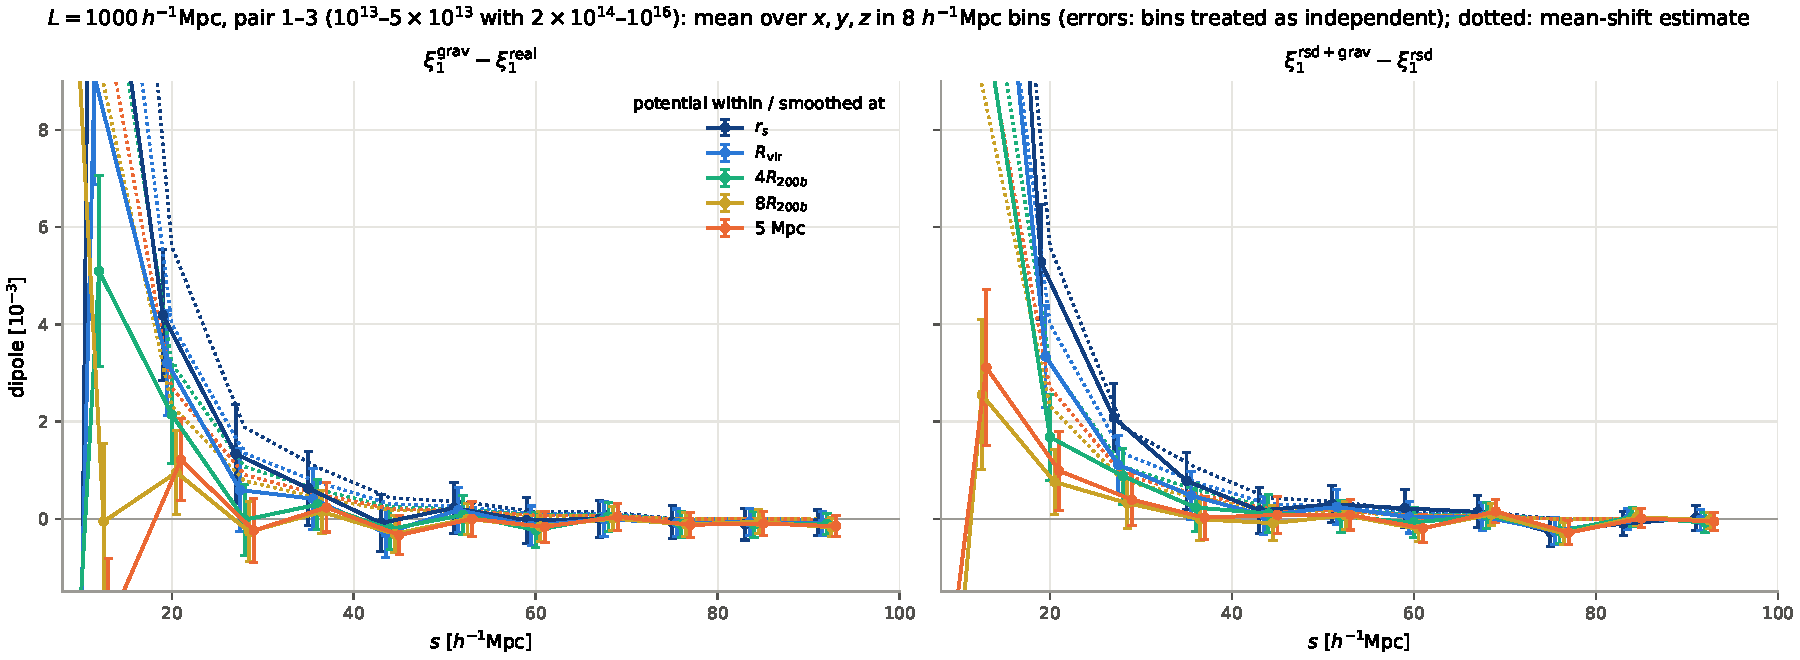
\includegraphics[width=\textwidth]{figs/ximult512_phi_s.pdf}
\caption{Dipole against $s$ in L1000 for pair 1--3 and five of the columns, in 8\,\Mpch{} bins; dotted: the
mean-shift estimate of each column. Below $\sim$8\,\Mpch{} halo exclusion dominates (not shown).}
\label{fig:ximult512_phi_s}
\end{figure}

\begin{table}[H]
\centering\footnotesize
% written by make_ximult_phi_figures.py
\begin{tabular}{lcccccc}
\toprule
potential & $\Delta v_g$ & \multicolumn{3}{c}{$\xi_1^{\rm grav}-\xi_1^{\rm real}$} & $\xi_1^{\rm rsd+grav}-\xi_1^{\rm rsd}$ & ratio \\
 & km\,s$^{-1}$ & L1000, 1–3 & L1000, 2–3 & L500, 0–3 & L1000, 1–3 & L1000, 1–3 \\
\midrule
$r_s$ & 13.0 & $+1.78\pm0.52$ (+2.50) & $+1.75\pm0.77$ (+2.36) & $+1.15\pm0.59$ (+1.88) & $+2.46\pm0.39$ (+2.36) & 0.71 \\
$0.5R_{\rm vir}$ & 10.8 & $+1.48\pm0.47$ (+2.07) & $+1.36\pm0.72$ (+1.91) & $+1.02\pm0.54$ (+1.66) & $+1.77\pm0.36$ (+1.90) & 0.72 \\
$R_{\rm vir}$ & 9.3 & $+1.18\pm0.43$ (+1.80) & $+1.00\pm0.65$ (+1.58) & $+0.76\pm0.48$ (+1.34) & $+1.44\pm0.34$ (+1.70) & 0.65 \\
$1.5R_{\rm vir}$ & 8.6 & $+1.00\pm0.41$ (+1.66) & $+0.91\pm0.64$ (+1.56) & $+0.66\pm0.46$ (+1.26) & $+1.31\pm0.33$ (+1.66) & 0.60 \\
$R_{200b}$ & 8.9 & $+1.08\pm0.42$ (+1.71) & $+0.95\pm0.65$ (+1.57) & $+0.64\pm0.47$ (+1.30) & $+1.34\pm0.34$ (+1.65) & 0.63 \\
\midrule
$2R_{200b}$ & 9.0 & $+1.14\pm0.42$ (+1.66) & $+0.88\pm0.65$ (+1.54) & $+0.67\pm0.48$ (+1.32) & $+1.43\pm0.34$ (+1.65) & 0.68 \\
$4R_{200b}$ & 7.4 & $+0.74\pm0.35$ (+1.28) & $+0.48\pm0.56$ (+1.28) & $+0.45\pm0.41$ (+1.10) & $+0.90\pm0.32$ (+1.43) & 0.57 \\
$6R_{200b}$ & 6.3 & $+0.46\pm0.32$ (+1.14) & $+0.30\pm0.47$ (+0.97) & $+0.21\pm0.37$ (+0.87) & $+0.56\pm0.30$ (+1.20) & 0.40 \\
$8R_{200b}$ & 5.4 & $+0.23\pm0.30$ (+0.99) & $+0.26\pm0.44$ (+0.87) & $+0.07\pm0.35$ (+0.78) & $+0.31\pm0.29$ (+1.12) & 0.23 \\
2 Mpc & 8.5 & $+1.03\pm0.41$ (+1.57) & $+0.96\pm0.63$ (+1.51) & $+0.64\pm0.45$ (+1.25) & $+1.23\pm0.33$ (+1.64) & 0.66 \\
3 Mpc & 7.7 & $+0.76\pm0.37$ (+1.40) & $+0.64\pm0.60$ (+1.44) & $+0.30\pm0.42$ (+1.09) & $+0.89\pm0.31$ (+1.44) & 0.54 \\
5 Mpc & 6.3 & $+0.28\pm0.33$ (+1.34) & $+0.34\pm0.50$ (+1.10) & $-0.14\pm0.37$ (+0.85) & $+0.29\pm0.30$ (+1.16) & 0.21 \\
\bottomrule
\end{tabular}

\caption{Dipole averaged over $s = 10$--$40$\,\Mpch{} in units of $10^{-3}$ for each potential column: measured
$\pm$ jackknife error (mean-shift estimate), for the best-measured pairs. $\Delta v_g = \langle v_g\rangle_3 - \langle
v_g\rangle_1$ in L1000. Ratio: measured over estimate for $\xi_1^{\rm grav}-\xi_1^{\rm real}$, L1000, pair 1--3.
Above the line: means within a sphere; below: smoothed grid.}
\label{tab:ximult512phi}
\end{table}

\paragraph{Results.} \emph{Mean $v_g$} (Fig.~\ref{fig:ximult512_phi_vg}): the potential within $r_s$ separates the
mass bins most; averaging over larger spheres, or smoothing the grid over larger radii, makes the halos of every bin
shallower and the difference between bins smaller. Between bins 1 and 3 in L1000 it falls from 13.0\,km\,s$^{-1}$
($r_s$) to 9.3 and 8.9 ($R_{\rm vir}$, $R_{200b}$) and 5.4 ($8R_{200b}$); the lowest bins hardly change (1.5--3.3\,km
s$^{-1}$). The grid at a fixed 2\,\Mpch{} is deeper than at $4$--$8R_{200b}$ for the top bin, whose $R_{200b}$ is
$\gtrsim1$\,\Mpch. \emph{Dipole} (Fig.~\ref{fig:ximult512_phi_dipole}, Table~\ref{tab:ximult512phi}): it follows
$\Delta v_g$, largest for $\phi_{r_s}$ and smallest for the widest apertures, in both differences and in every box
and pair where it is measured. In L1000, pair 1--3, $\xi_1^{\rm grav}-\xi_1^{\rm real}$ goes from
$(1.78\pm0.52)\times10^{-3}$ ($r_s$, 3.4$\sigma$) through $(1.08\pm0.42)\times10^{-3}$ ($R_{200b}$) to
$(0.23\pm0.30)\times10^{-3}$ ($8R_{200b}$); with redshift-space distortions, $(2.46\pm0.39)\times10^{-3}$ to
$(0.31\pm0.29)\times10^{-3}$. \emph{Against the mean-shift estimate}: for the five spheres and the grid at $2R_{200b}$
and 2\,\Mpch{} the measured dipole is 0.6--0.7 of the estimate ($\xi_1^{\rm grav}-\xi_1^{\rm real}$; 0.75--1.04 with
redshift-space distortions), for the widest apertures much less: 0.40 at $6R_{200b}$, 0.23 at $8R_{200b}$, 0.21 at
5\,\Mpch{} (0.47, 0.27, 0.25). Fig.~\ref{fig:ximult512_phi_s} shows where: at $s\approx10$--25\,\Mpch{} the dipole of
the wide apertures stays far below their estimates, while those of $\phi_{r_s}$ and $\phi_{R_{\rm vir}}$ follow theirs.
A likely reading (not tested further here): a potential smoothed over $\sim$10\,\Mpch{} contains the large-scale
potential of the environment, which two halos 10--25\,\Mpch{} apart largely share, so it shifts them alike and leaves
less relative shift than the bin means suggest; the mean-shift estimate ignores this. \emph{Caveats}: one realisation
per box at $z=0$; L200's top bin (76 halos) and L1000's lowest bin (3--15 particles per halo) are not usable for this;
the errors treat the 2\,\Mpch{} bins as independent.
